\section{Plan de verificación, resultados y evidencias}
\subsection{Pruebas de módulo ejecutadas}
Se diseñaron pruebas unitarias sobre la lógica criptográfica y la persistencia; se ejecutaron en el entorno de preparación del proyecto. Resultado observado: \textbf{20 pruebas aprobadas}. Entre los casos están los siguientes:

\begin{longtable}{p{4.2cm}p{8.9cm}}
\toprule Caso & Resultado esperado\\\midrule\endhead
Inicio de sesión correcto e incorrecto & Aceptar sólo la contraseña que verifica el hash Argon2id.\\
Reversibilidad AES + RSA & Descifrar la misma candidatura que fue cifrada.\\
Manipular ciphertext o nonce & Rechazo por error de autenticación AES-GCM.\\
Sobre inválido & Rechazo por estructura, Base64 o tamaños incorrectos.\\
Dos votos con una misma cuenta & Aceptar primero, rechazar segundo.\\
Dos envíos concurrentes & Solamente una transacción exitosa.\\
Cuenta inexistente & El sistema rechaza el intento.\\
Modificar tabla de boletas & Auditoría de cadena falla.\\
Cierre de elección & No se aceptan más votos.\\
Tally y firma & Se cuentan 2 votos A, 1 B, 0 C y se valida Ed25519.\\
Alterar conteos firmados & La verificación de firma falla.\\
Cambio de la cadena publicada & La auditoría devuelve falso.\\
Cifrado JS/Python & Una boleta cifrada con Web Crypto (Node) es descifrable en Python.\\
\bottomrule
\end{longtable}

\subsection{Demostración de escrutinio desde la terminal}
En una ejecución aislada con tres cuentas de prueba, se registraron las selecciones A, C y A; después de cerrar la elección, el programa generó un resultado de \textbf{2 votos para A, 0 para B y 1 para C}, sin boletas inválidas. La verificación de la firma Ed25519 y de la cadena devolvió un estado válido. Esta ejecución corresponde a datos ficticios generados para la validación del software.


\subsection{Capturas}
\textbf{> Inicio de sesión}
\newline
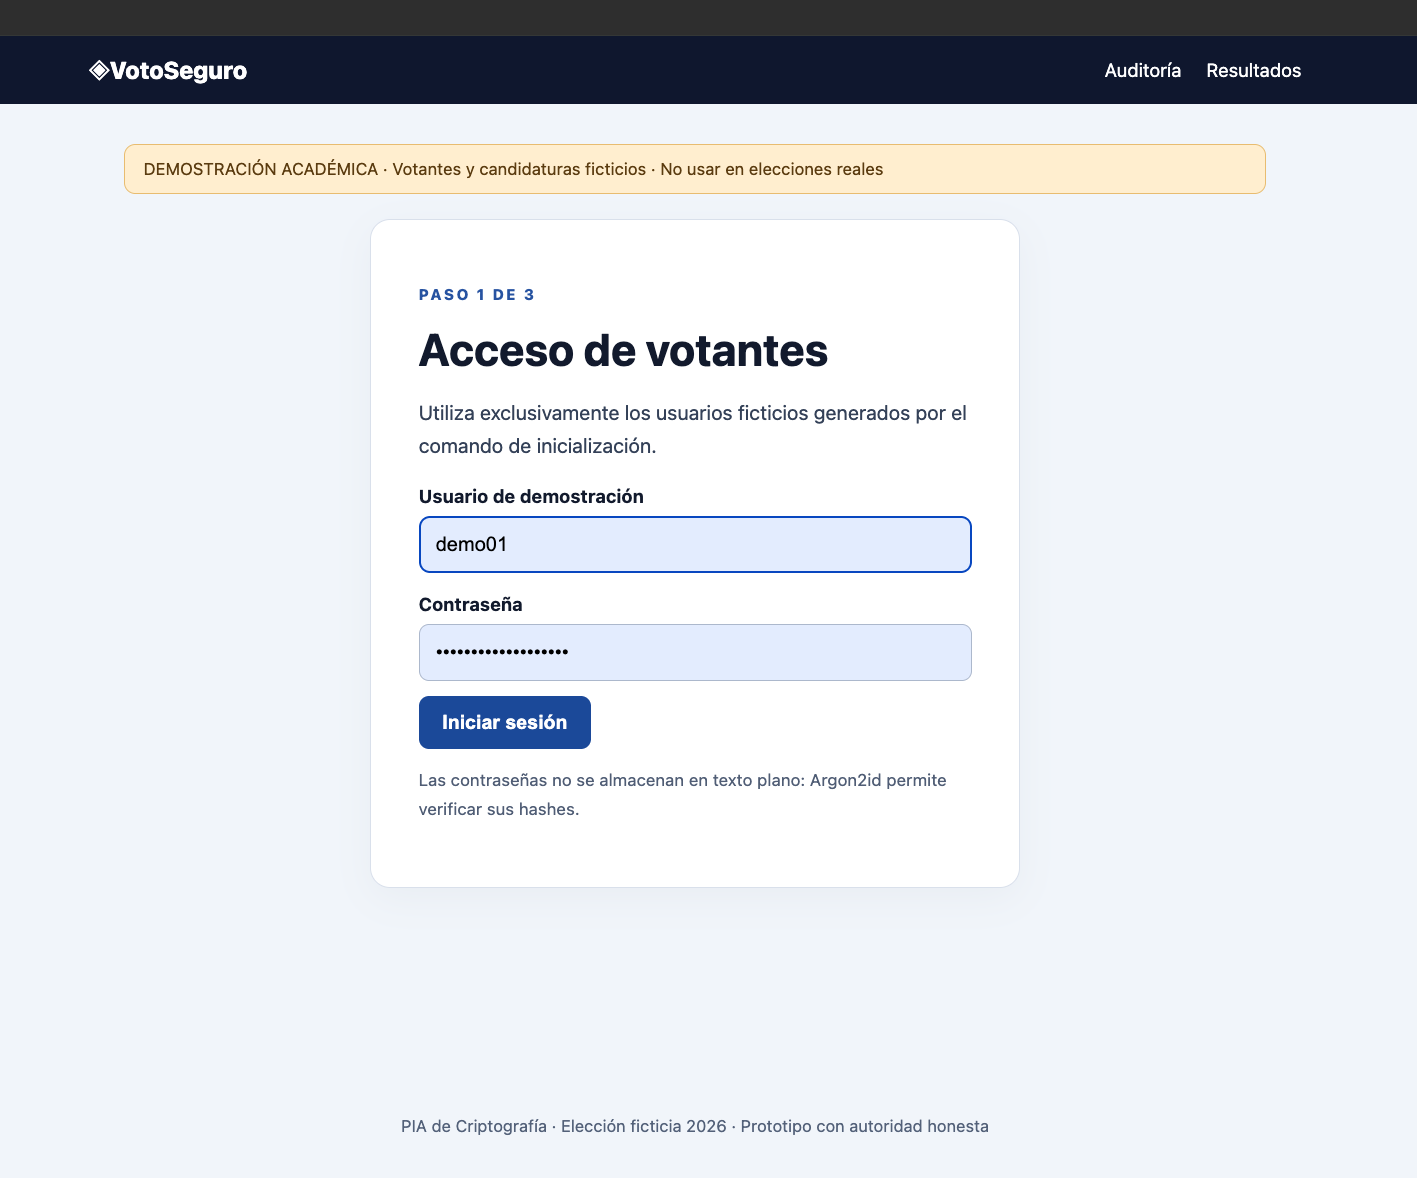
\includegraphics[width=.85\linewidth]{docs/evidencias/Formulario de inicio de sesión con usuario ficticio.png}

\newpage
\textbf{Menú de selección (3 candidatos)}
\newline
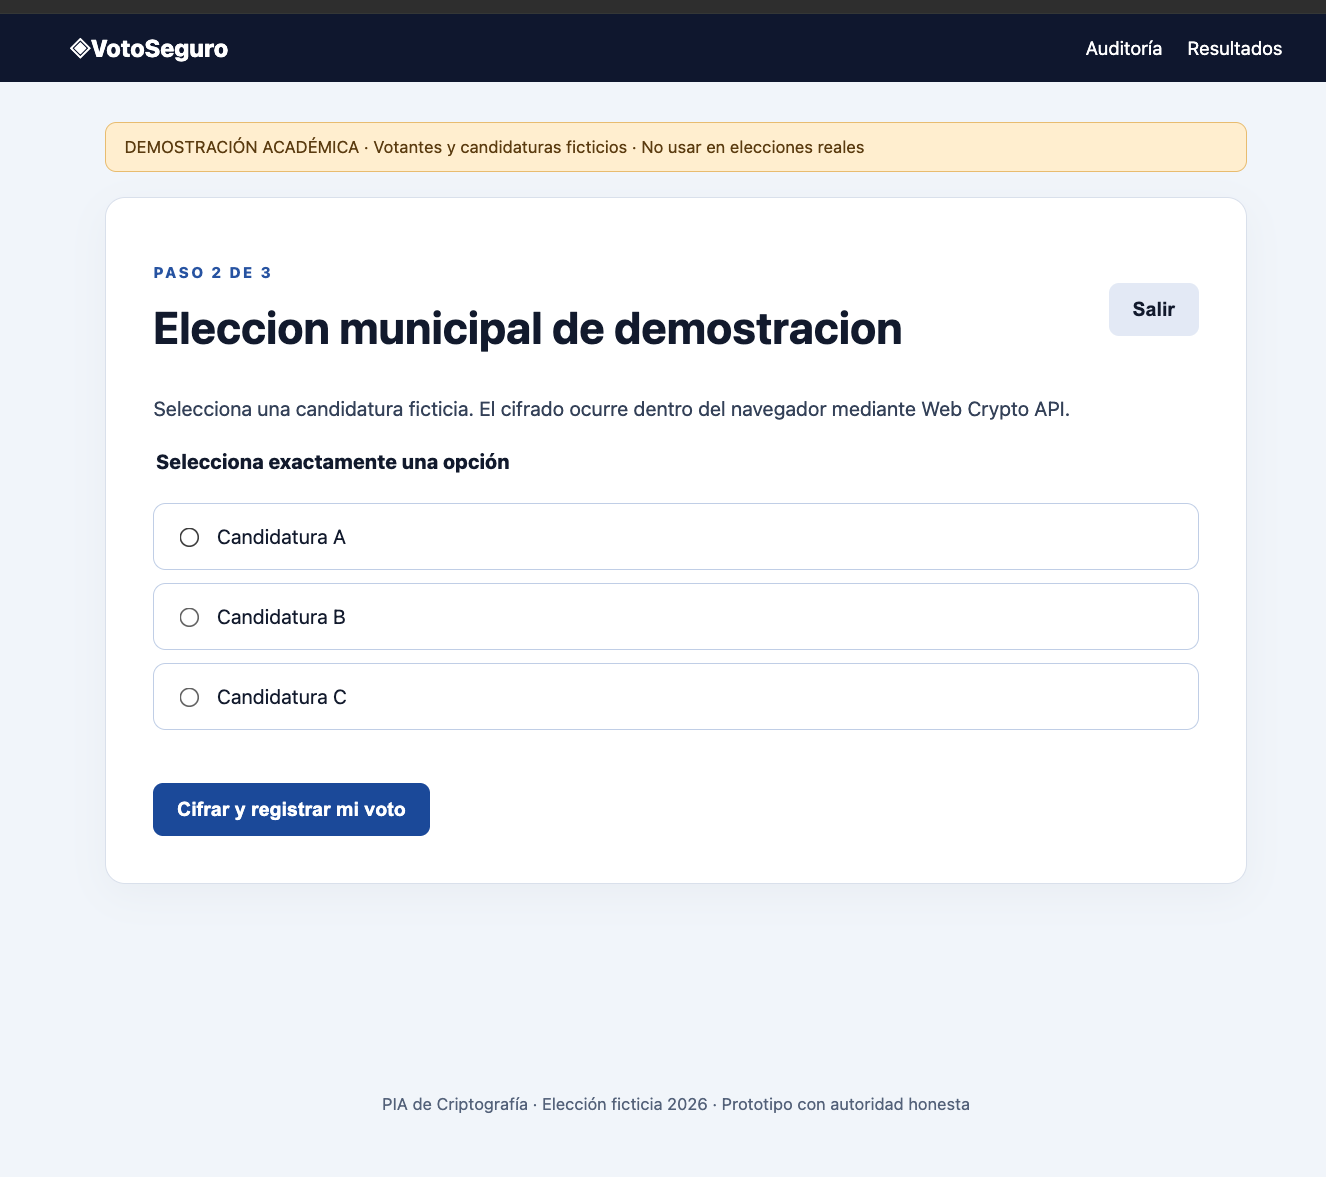
\includegraphics[width=.85\linewidth]{docs/evidencias/Boleta con 3 candidaturas ficticias.png}

\newpage
\textbf{Selección de uno de los 3 candidatos}
\newline
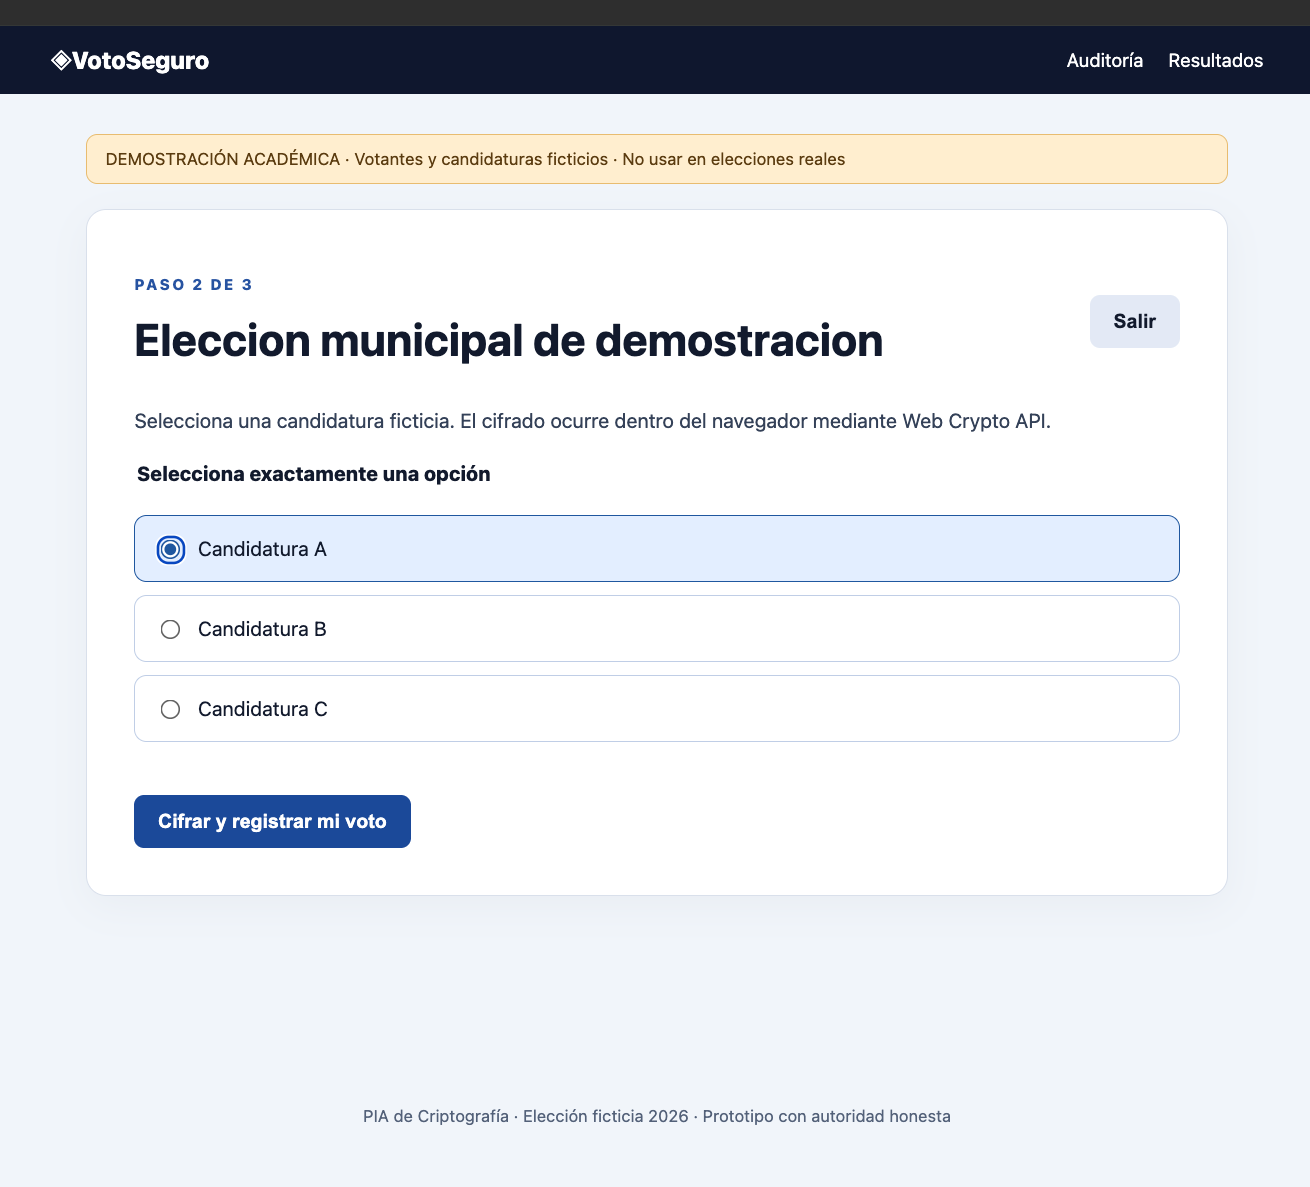
\includegraphics[width=.85\linewidth]{docs/evidencias/Boleta con la candidatura A seleccionada.png}

\newpage
\textbf{Comprobante de registro}
\newline
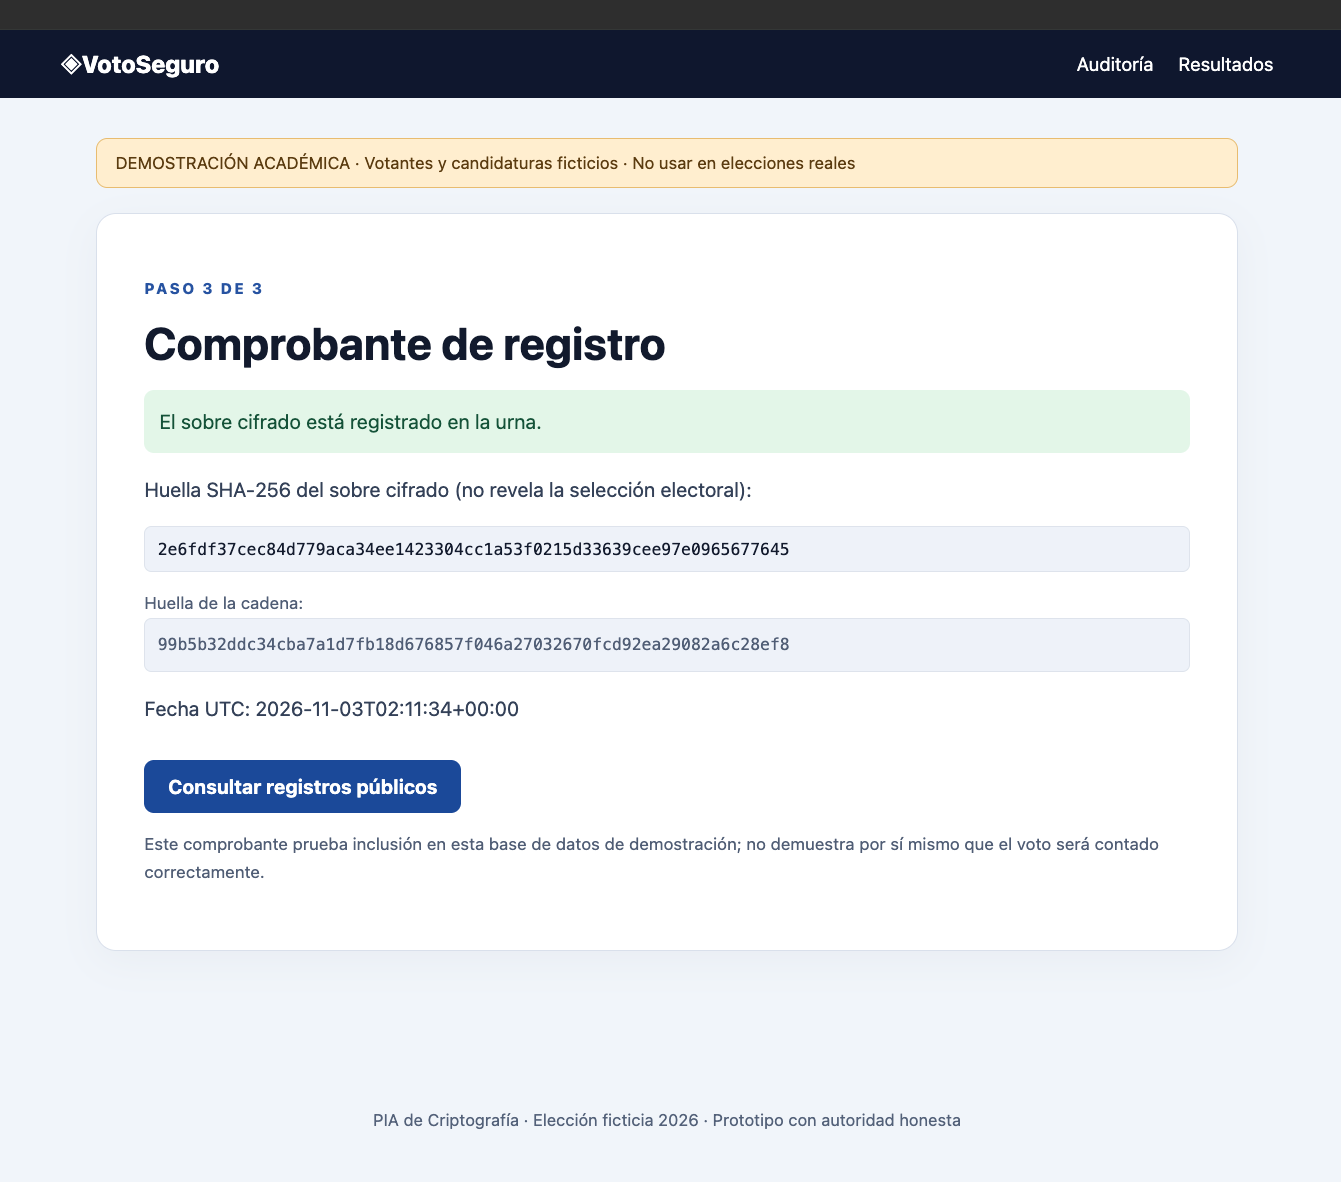
\includegraphics[width=.85\linewidth]{docs/evidencias/Comprobante con voto firmado.png}

\newpage
\textbf{Prohibición al querer votar de nuevo desde una cuenta que ya voto antes}
\newline
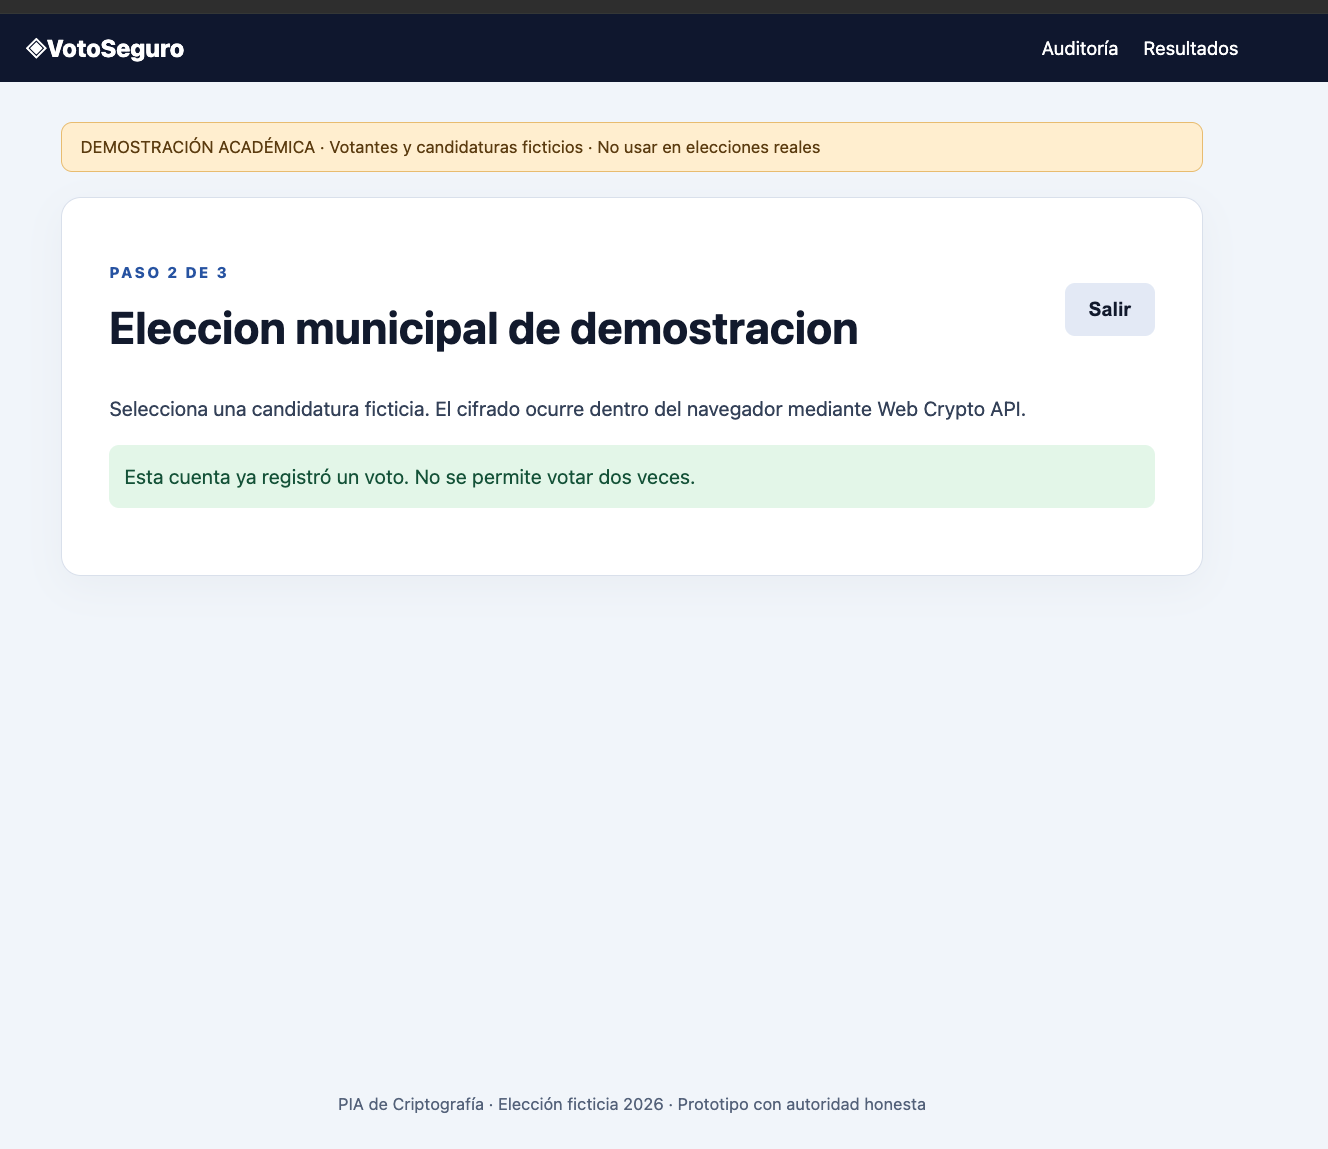
\includegraphics[width=.85\linewidth]{docs/evidencias/Intento rechzado.png}

\textbf{Prueba de escrutinio (urna aun abierta)}
\newline
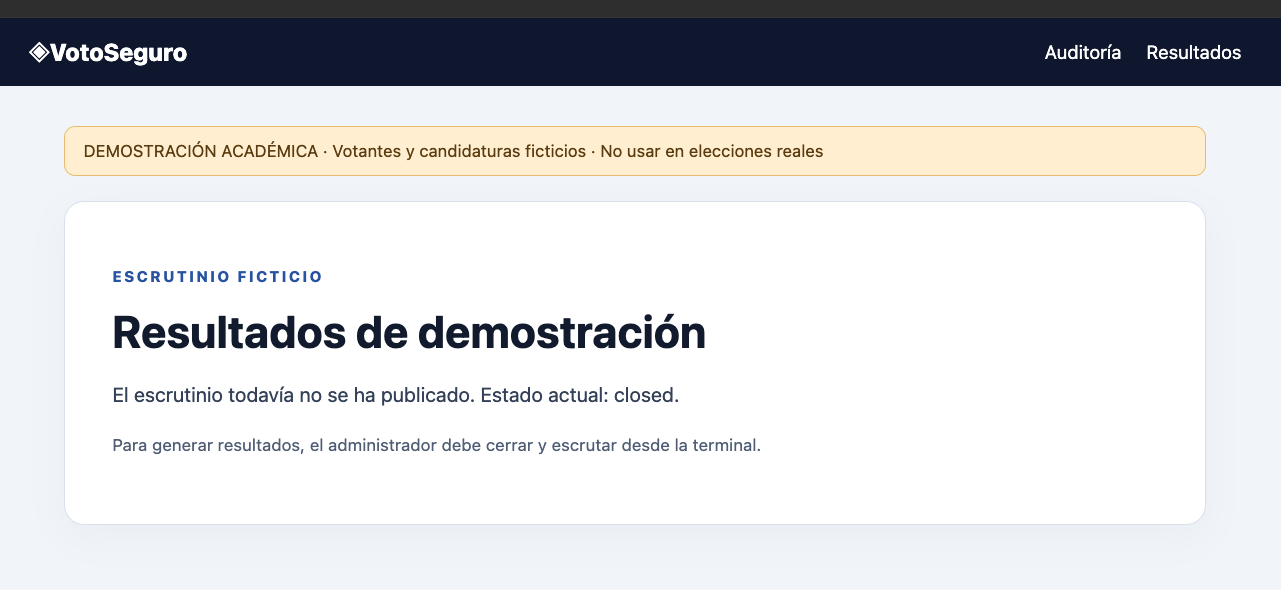
\includegraphics[width=.85\linewidth]{docs/evidencias/urna cerrda.png}

\newpage
\textbf{Prueba de los 5 votos de las 5 cuentas}
\newline
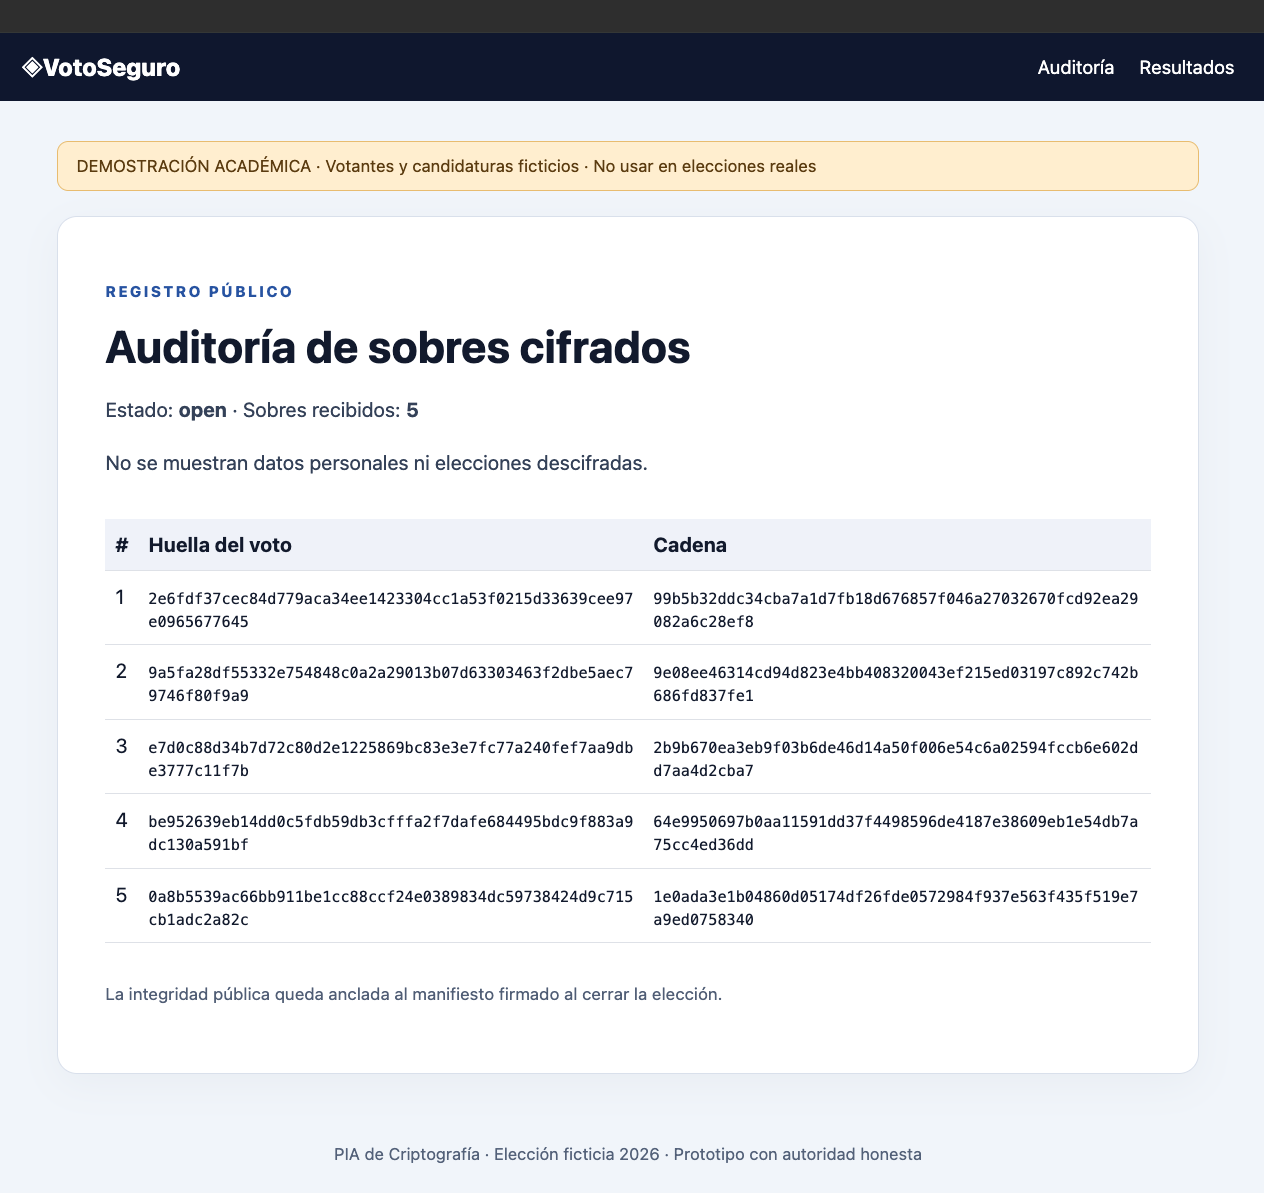
\includegraphics[width=.85\linewidth]{docs/evidencias/5 votos.png}

\newpage
\textbf{Prueba del resultado final}
\newline
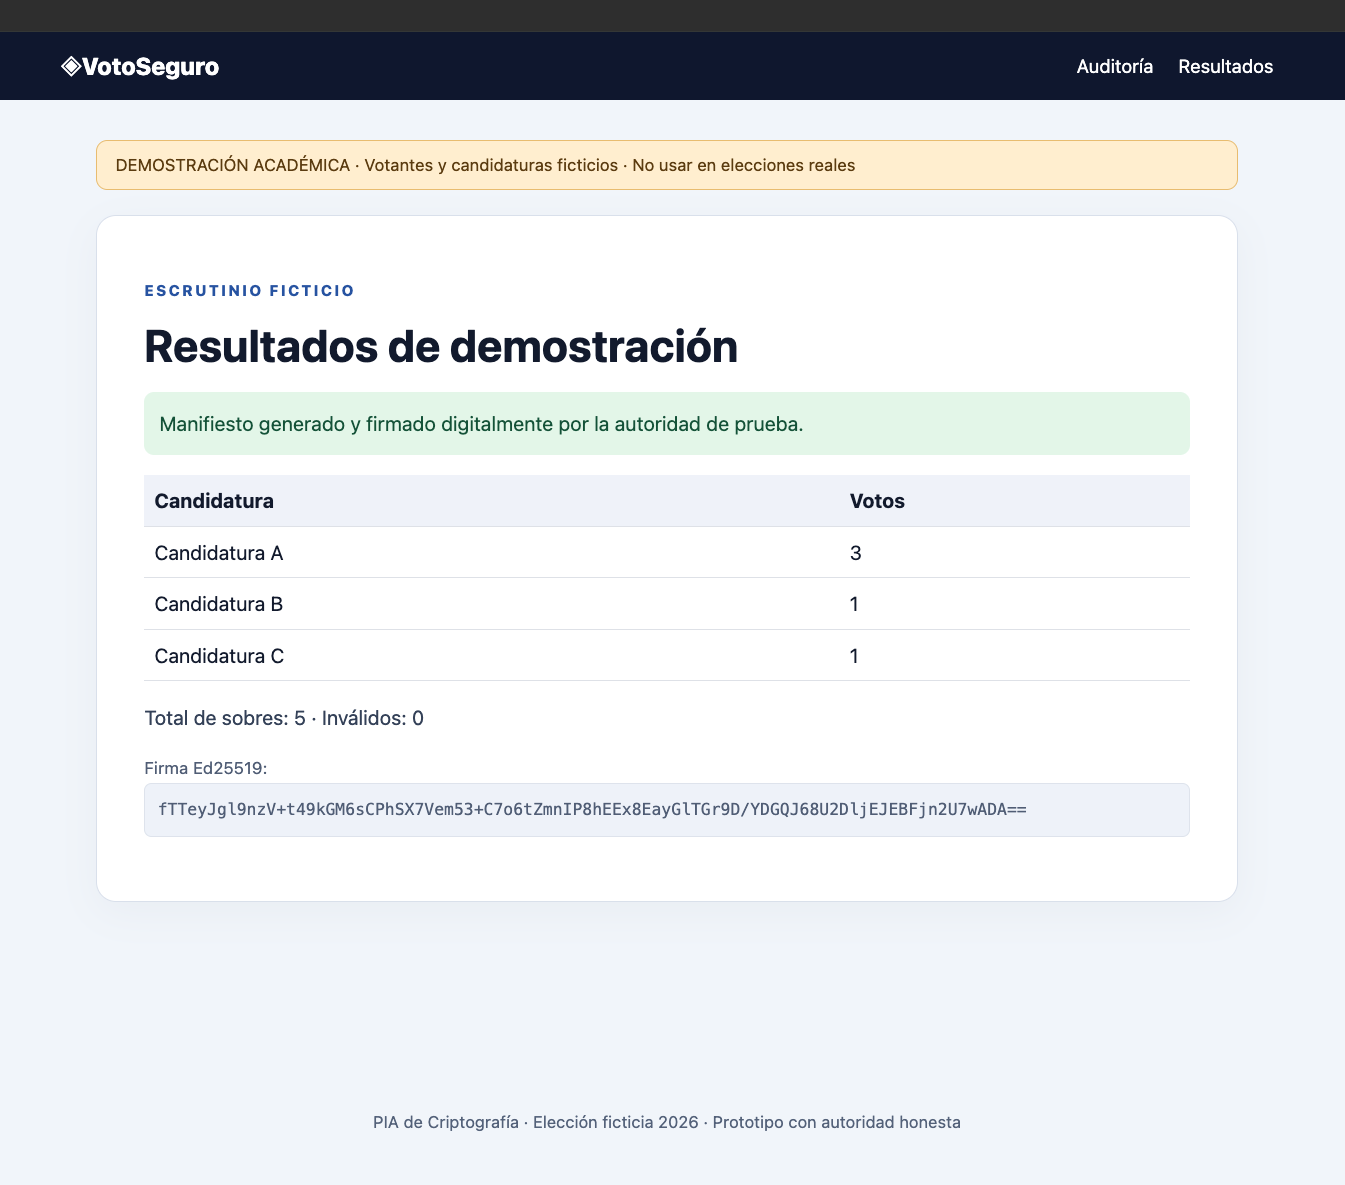
\includegraphics[width=.85\linewidth]{docs/evidencias/Firma final y resultados.png}

\textbf{Prueba de la terminal de comandos y de la validación de cadenas y firma}
\newline
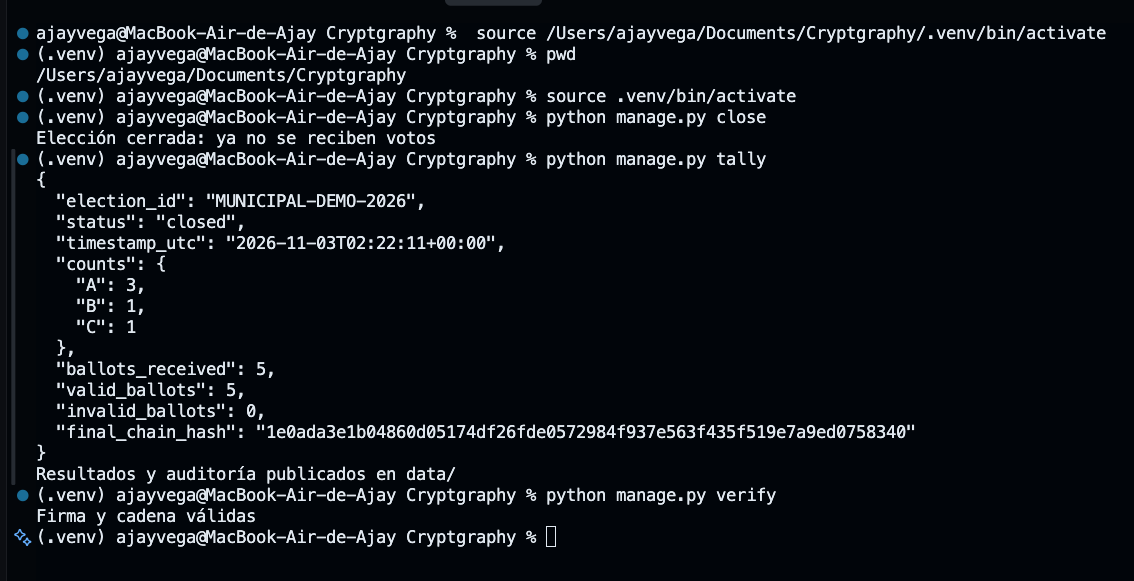
\includegraphics[width=.85\linewidth]{docs/evidencias/Terminal con proceso.png}
%--
%--\missingimage{Formulario de inicio de sesión con usuario ficticio }
%--\missingimage{la boleta y tres candidaturas ficticias}
%--\missingimage{el fckin comprobante SHA-256 de un voto confirmado}
%--\missingimage{y un ntento repetido y rechazo del sistema}
%--\missingimage{la auditoria, resultados y la terminal con pytest}

% NIGGAAA, Para sustituir cada recuadro en Overleaf, subir la captura a la carpeta \code{evidencias/} y reemplazar la instrucción \code{\\missingimage\{...\}} por \code{\\includegraphics[width=.85\\linewidth]\{evidencias/nombre.png\}}.

% nigga thx
